\documentclass[a4paper,10pt,ngerman]{scrartcl}
\usepackage{babel}
\usepackage[T1]{fontenc}
\usepackage[utf8x]{inputenc}
\usepackage[a4paper,margin=2.5cm,footskip=0.5cm]{geometry}

\usepackage{hyperref}

% Die nächsten drei Felder bitte anpassen:
\newcommand{\Aufgabe}{Physik GFS - Schaltkreise} % Aufgabennummer und Aufgabennamen angeben
\newcommand{\Name}{Lars Noack}             % Name des Bearbeiter / der Bearbeiterin dieser Aufgabe angeben


% Kopf- und Fußzeilen
\usepackage{scrlayer-scrpage, lastpage}
\setkomafont{pageheadfoot}{\large\textrm}
\lohead{\Aufgabe}
\cfoot*{\thepage{}/\pageref{LastPage}}

% Position des Titels
\usepackage{titling}
\setlength{\droptitle}{-1.0cm}

% Fuer mathematische Befehle und Symbole
\usepackage{amsmath}
\usepackage{amssymb}

% Fuer Bilder
\usepackage{graphicx}

% Fuer Algorithmen
\usepackage{algpseudocode}

% Fuer Quelltext
\usepackage{listings}
\usepackage{color}
\definecolor{mygreen}{rgb}{0,0.6,0}
\definecolor{mygray}{rgb}{0.5,0.5,0.5}
\definecolor{mymauve}{rgb}{0.58,0,0.82}
\lstset{
  keywordstyle=\color{blue},commentstyle=\color{mygreen},
  stringstyle=\color{mymauve},rulecolor=\color{black},
  basicstyle=\footnotesize\ttfamily,numberstyle=\tiny\color{mygray},
  captionpos=b, % sets the caption-position to bottom
  keepspaces=true, % keeps spaces in text
  numbers=left, numbersep=5pt, showspaces=false,showstringspaces=true,
  showtabs=false, stepnumber=2, tabsize=2, title=\lstname
}
\lstdefinelanguage{JavaScript}{ % JavaScript ist als einzige Sprache noch nicht vordefiniert
  keywords={break, case, catch, continue, debugger, default, delete, do, else, finally, for, function, if, in, instanceof, new, return, switch, this, throw, try, typeof, var, void, while, with},
  morecomment=[l]{//},
  morecomment=[s]{/*}{*/},
  morestring=[b]',
  morestring=[b]",
  sensitive=true
}

\lstset{language=Python}
\lstset{frame=lines}
\lstset{caption={Sprache: Python}}
\lstset{label={lst:code_direct}}
\lstset{basicstyle=\footnotesize}

% Diese beiden Pakete muessen zuletzt geladen werden
%\usepackage{hyperref} % Anklickbare Links im Dokument
\usepackage{cleveref}

% Daten fuer die Titelseite
\title{\textbf{\Huge\Aufgabe}}
\author{\LARGE Name: \\ 
	    \LARGE \Name\\\\}
\date{\LARGE\today}

\begin{document}

\maketitle

\setcounter{tocdepth}{5}
\tableofcontents

\vspace{0.5cm}

Ich gehe davon aus, dass die Aufgabe klar ist, sonst geht diese aus der Projektsite heraus.

\section{Physikalische Grundlagen}
\label{subsec:physik}

Wir wollen die Stromstärke, Spannung und den Widerstand aller Widerstände und Teilwiderstände in einer Schaltung berechnen. Dafuer brauchen wir Formeln.

\subsection{Ohmsches Gesetz}

Das Ohmsche Gesetz beschreibt den Zusammenhang von Stromstärke, Spannung und dem Widerstand in einem Widerstand bzw in einem Teilwiderstand.

Wenn $R = Konstant$ dann $U \sim I$

Die Formel dafür lautet $U = R \cdot I$ und kann umgeschrieben werden als $R = \frac{U}{I}$ und in $I = \frac{U}{R}$

\subsection{Kirchofsche Regeln}

Die Kirchofsche Regeln sind ein Set von Regeln, bestehend aus 2 Regeln, der Knotenregel und der Maschenregel. Diese beschreiben das Verhalten von Stromstärke bzw. Spannung in Reihen- bzw. Parrallelschaltungen, unabhängig vom Widerstand.

\paragraph{Knotenregel}

Die Knotenregel besagt, dass die Spannung bei Knoten gleich ist. Ein Knoten bezeichnet in dem Fall eine Parrallelschaltung. Vereinfacht sagt die Regel, dass alle Teilwiderstände in einer Parrallelschaltung die gleiche Spannung haben.

$U_{ges} = U_1 = U_2 = U_3 = U_4 = ...$

\paragraph{Maschenregel}

Die Maschenregel besagt, dass die Stromstärke bei allen Maschen gleich ist. Als eine Masche bezeichnet man hier eine Reihenschaltung. Vereinfacht sagt die Regel, dass alle Teilwiderstände in einer Reihenschaltung die gleichen Stromstärken haben.

$I_{ges} = I_1 = I_2 = I_3 = I_4 =...$

\subsection{Widerstände in einer Reihenschaltung}

Dies beschreibt das Verhalten der Stromstärke, der Spannung und des Widerstandes in einer Reihenschaltung.

\paragraph{Spannung}

$U_{ges} = U_1 + U_2 + U_3 + U_4 +...$

\paragraph{Widerstand}

$R_{ges} = R_1 + R_2 + R_3 + R_4 +...$

\subsection{Widerstände in einer Parrallelschaltung}

Dies beschreibt das Verhalten von der Stromstärke, der Spannung und des Widerstandes in einer Parrallelschaltung.

\paragraph{Stromstärke}

$I_{ges} = I_1 + I_2 + I_3 + I_4 +...$

\paragraph{Widerstand}

$\frac{1}{R_{ges}} = \frac{1}{R_{1}} + \frac{1}{R_{2}} + \frac{1}{R_{3}} + \frac{1}{R_{4}} +...$

\section{Repräsentation eines Schaltkreises als Baum}

\subsection{Die Schaltung als ungerichteter Graph}

Eine Widerstand-Schaltung ist ein Graph. Also ein Netz aus Knoten, die mit Kanten verbunden sind. Die Knoten repräsentieren die Widerstände, wobei die Kanten die Verbindungen zwischen den Widerständen repräsentieren.
Eigentlich ist der Graph ein gerichteter Graph, da der Strom nur in eine Richtung fließt. Jedoch ist die Fließrichtung für dieses Projekt irrelevant, wodurch wir auch einen ungerichteten Graphen nehmen koennen.\footnote{Ein Graph ist gerichtet, wenn die Kanten nur in eine Richtung gehen und ungerichtet, wenn sie in beide Richtungen gehen. \url{https://de.wikipedia.org/wiki/Gerichteter_Graph}}

\subsection{Die Schaltung als Baum}
\label{subsec:baum}

Ein Baum ist eine Datenstruktur in der Informatik. Der unterschied zu einem Graph ist, dass ein Baum hierarchisch angeordnet ist und von oben nach unten geht. Also koennen auch bei einem ungerichteten Baum untere Knoten sich nicht mehr mit den Oberen verbinden

\url{https://de.wikipedia.org/wiki/Baum_(Datenstruktur)}

\includegraphics[width=0.5\textwidth]{circuit3.png}

Jetzt ist eine Schaltung so aber noch kein Baum, da sich ein Schaltkreis immer in einem Kreis schließt, was bei einem Baum verboten ist. Um aber zu erklären, wie ein Baum jede Widerstand-Schaltung repräsentieren kann, ziehe ich ein Beispiel hinzu (oben)\footnote{Die Grafik hat mein Programm generiert}.

Die Wurzel des Baumes \footnote{Der oberste Knoten} ist eine Reihenschaltung. Dieser hat die Kinder $R_1$ und $R_2, R_3$ welche die Teilwiderstände in der Reihenschaltung sind.

$R_2, R_3$, das Kind der Wurzel, ist eine Parrallelschaltung mit den Kindern $R_2$ und $R_3$.

Dies kann man bis ins unendlich Komplexe skalieren.

\includegraphics[width=.7\textwidth]{baum.png}

So würde der Baum dann aussehen.

\section{die Eingabe des Schaltkreises}

\subsection{Speichern des Baums in einer Adjazenzliste}

Graphen und Bäume werden häufig in einer Adjazenzliste gespeichert. Das heißt, man schreibt die Knoten, die von einer Kante verbunden sind, nebeneinander. Um besser zu beschreiben, was eine Adjazenzliste ist, ziehe ich das obere Beispiel des Baumes hinzu und erstelle die Adjazenzliste davon.\footnote{Dies ist ein CSV comma seperated format, das heißt die Knoten sind von einem Komma getrennt.}

\begin{flushleft}
Reihenschaltung R123, Widerstand R1\\
Reihenschaltung R123, Parralelschaltung R23\\
Parralelschaltung R23, Widerstand R2\\
Parralelschaltung R23, Widerstand R3\\
\end{flushleft}

\subsection{Eigentliche Eingabe}

Jetzt reicht für die Eingabe keine einfache Adjazenzliste, da man nicht nur die Widerstände und Schaltungen
angeben muss, sondern auch die angegebenen Werte der Widerstände und die der Teilwiderstände. Das heißt, ich brauche ein Separator zwischen
den Knoten, und einen Separator, um die angegebenen Werte in den Knoten von den jeweiligen Verbindungsknoten zu unterscheiden.

Als Separator für die Koten habe ich eine freie Zeile verwendet. Um in einem Knoten zwischen angegebenem Wert und Verbindung zu unterscheiden, rückt man die angegebenen Werte ein, und die Verbindungen nicht.

\subsection{Details der Implementierung}

\begin{itemize}

\item Wenn man einen Kommentar\footnote{Text, den mein Programm ignoriert um etwas zu beschreiben} hinzufügen will macht man dass mit '//', inspiriert von Programmiersprachen wie C, C++, Java, JavaScript....
\item Um den Typ eines Knoten anzugeben, schreibt man in der ersten Zeile nach dem Namen hinter dem Komma entweder R (resistor), P (parallel), S (series) 
\item Man muss nicht jeden Knoten angeben. Wenn der Knoten nur in einer Verbindung eines anderen Knoten erwähnt wird, wird angenommen, dieser Knoten ein Widerstand ohne angegebene Werte ist.
\item Man muss nicht bei jedem Knoten alle Werte hinschreiben oder explizit erwähnen die fehlen, man muss lediglich z.B. R: 10 hinschreiben und dann weiß mein Programm, dass lediglich der Widerstand mit 10 Ohm angegeben wurde.
\item Diesen Text kann man in eine Datei schreiben und diese auslesen lassen, oder direkt in das Programm.

\end{itemize}

\subsection{Beispiel}

\begin{verbatim}
// Kommentar der Ignoriert wird.
Rges, S
    U: 24
R1
R23

R23, P
R2
R3

R2, R
    R: 40

R3, R
    R: 60
    I: 0.3
\end{verbatim}

\section{Das Einlesen der Liste}

Vorab, der Code des Programmes der dies macht ist \hyperref[subsec:verarbeitung]{\underline{hier}} zu finden.

\noindent Aber bevor ich darauf eingehe wie ich die Liste einlese, muss ich erstmal kurz erklären was Klassen sind.

\subsection{Klassen}

Eine Klasse ist ein Container. In diesem Container können Variablen oder Listen gespeichert werden, Programmcode stehen, der diese Variablen oder Listen bearbeitet, und vieles mehr auf das ich nicht in Tiefe eingehen kann.
Was ich also gemacht habe ist, dass jeder Knoten eine Instanz einer Klasse ist, in der eine Liste weiterer Knoten (den untergeordneten Knoten) ist.

Dies vereinfacht die Verarbeitung der Daten immens.

\subsection{Die gewünste Klassenstruktur erhalten}

\begin{itemize}
\item Um jetzt aber diese Klassenstruktur zu erhalten, gehe ich erst einmal mit einer Schleife jeden Knoten der Datei durch.
\item Bei jedem Knoten schaue ich, ob ich ihn schon unter dem Namen in der Liste abgespeichert habe.
\item Wenn ich dies habe, ändere ich trotzdem die Art des Knotens zu der, die in der Datei angegeben ist. (Das wird Sinn machen)
\item Wenn dies nicht so ist, dann speichere den Namen unter dem jeweiligen Typ.
\item Dann speichere ich alle angegebenen Werte unter dem Namen des jeweiligen Knoten.
\item Der letzte wichtige Schritt ist das Durchgehen aller angegebenen Verbindungen des jeweiligen Knotens.
\item Dabei speichere jede Verbindung ab, schaue aber auch, ob der Name des verbundenen Knotens schon abgespeichert ist.
\item Sollte dies nicht der Fall sein, dann speichere ich ihn unter dem Typ Widerstand ohne Werte ab.\footnote{Deshalb war es auch wichtig bei jedem angegebenen Knoten den Typ zu ändern, ist der Knoten schon abgespeichert.}
\end{itemize}

Dann kann man diese Klassen einfach erstellen.

Wenn dieser Programmstruktur nicht gefolgt werden konnte, ist dies nicht schlimm sondern verständlich. Aber um nochmal zusammenzufassen:

jetzt haben wir diesen  \hyperref[subsec:baum]{\underline{Baum}}, und können mit ihm arbeiten

\section{Des Rendern des Schaltplans}

Dies war ein absolut notwendiger Schritt, da man sonst keine Möglichkeit hat zu überprüfen, ob der Schaltkreis richtig eingegeben wurde.

\subsection{schemdraw}

Ursprünglich wollte ich dieses Programm als Website machen, hab ich dann nicht gemacht, da ich für das Web bzw. JavaScript nur eine Library\footnote{Code, den andere geschrieben haben.} gefunden habe,
bei der das Beispielprogramm 1000 Zeilen lang war. Für Python habe ich eine schönere Library gefunden, \href{https://pypi.org/project/schemdraw/}{\underline{schemdraw}}.

Mit ihr konnte ich ein Objekt erstellen, und dann zu dem Objekt verschiedene Elemente wie Stromquelle, Widerstände, Kondensatoren, etc. hinzufügen, bei dem ich aber nur Widerstände und eine Stromquelle verwendet habe.

Dann konnte ich das als svg exportieren und musste es dann in png umwandeln.\footnote{das hat soooo viele Stunden gebraucht.}

\includegraphics[width=0.5\textwidth]{circuit3.png}

\subsection{Implementierung}

Auch wenn diese sehr simpel zu erklären ist, war sie unglaublich schwer zu programmieren.

Als erstes habe ich ein Schemdraw Objekt erstellt. Dann habe ich dies der Wurzel gegeben. Wenn ein Knoten dann dieses Objekt bekommen hat, hat dieser, wenn er ein Widerstand ist, einfach ein Widerstand hinzugefügt. Ist dieser aber eine Reihen- oder Parallelschaltung, dann gibt er das Objekt an alle Kinder weiter, und zeichnet dann nur die Verbindungen zwischen den zurückgegebenen Änderungen.

Der Grund warum das soooooo schwer war, waren die vielen edge cases, zum Beispiel woher der Knoten weiß wie lang die Verbindungslinien sein sollen.

\section{Berechnung der fehlenden Werte}

Vorab, der Programmcode dazu ist \hyperref[subsec:berechnung]{\underline{hier}} zu finden.

Für so etwas existiert kein Algorithmus, der bekannt ist. Deshalb musste ich meinen eigenen machen. Mein Algorithmus weist jedoch Ähnlichkeiten zum \href{https://en.wikipedia.org/wiki/Bellman\%E2\%80\%93Ford_algorithm}{\underline{Bellman-Ford}} Algorithmus\footnote{Ein Algorithmus zum Finden des kürzesten Weges, der häufig im Netzwerkrouting verwendet wird, also etwas ganz anderes macht.}auf.
Bei Bellman-Ford werden immer benachbarte Knoten 'geupdated', wenn sich der Wert eines Knoten verändert. Ich mache das prinzipiell genauso.

\subsection{Basis}

Nur nochmal zur Erinnerung. Ein Knoten kann sowol ein Widerstand, als auch eine Parallelschaltung oder Reihenschaltung sein. Wenn er eine Schaltung ist, hat er mehr als 1 Kinder\footnote{1 Kind wäre möglich aber sinnlos}, und wenn der Knoten ein Widerstand ist, hat er kein Kind.
Als erstes betrachtet mein Programm die Wurzel. Hier wird dann zuerst\footnote{Wenn der Knoten eine Schaltung ist} für alle 3 Werte\footnote{U, R, I} die Anzahl an Kindern herausgefunden, bei denen dieser Wert fehlt. Wenn bei einem der Werte nur 1 Wert fehlt (Eingenommen dem der Wurzel), so wird dieser je nach Schaltung berechnet. Wie das berechnet wird, wurde schon in \hyperref[subsec:physik]{\underline{Physikalische Grundlagen}} gesagt.
Dann wird nach der Maschen- bzw. Knotenregel sowol bei sich selbst geschaut ob dort etwas gemacht werden kann, als auch bei allen Kindern. Anschließend wird auch geprüft, ob man mit dem Ohmschen Gesetz etwas berechnen kann, und ggf. wird der Wert dann berechnet.

Dann wird jedes Kind des Knotens aufgefordert das Gleiche zu machen (außer der Knoten ist ein Widerstand). \textbf{Das stellt sicher, dass das, solange alle Widerstände mit der Wurzel verbunden sind, mit jedem durchgeführt wird.}

\subsection{Warum lässt der Algorithmus nichts aus?}

Der Grund warum der Algorithmus funktioniert, ist dass jeder Knoten bei jeder Änderung eines Wertes alle obrigen Schritte macht, und somit alle Werte, die mit der Änderung dieses einen Werts noch berechnen werden können, auch berechnet werden. Hier ist auch die Ähnlickeit zum Bellman-Ford Algorithmus - sie ist aber ziemlich gering.

Natürlich prüfe ich nicht immer alle Regeln, das wäre vergleichsweise ineffizient, sondern prüfe die nur dann wenn es Sinn macht. Das aber genau zu beschreiben würde hier einfach den Rahmen sprengen.

\newpage
\section{Beispiel}

Bis auf das Beispiel um die Komplexität zu testen, habe ich die Beispiele von \url{https://ulrich-rapp.de/stoff/fahrzeug/daten/ET_Ub_Ohm.pdf} genutzt, da man sich keine Fehler in der Aufgabe erlauben \textbf{DARF}, da sonst Werte falsch sind.

\subsection{Komplexer Schaltkreis}

Dies ist ein Beispiel ohne Werte, um zu zeigen, wie komplex die Schaltkreise werden können. Sie können sogar noch komplexer werden und mein Programm kommt damit klar.

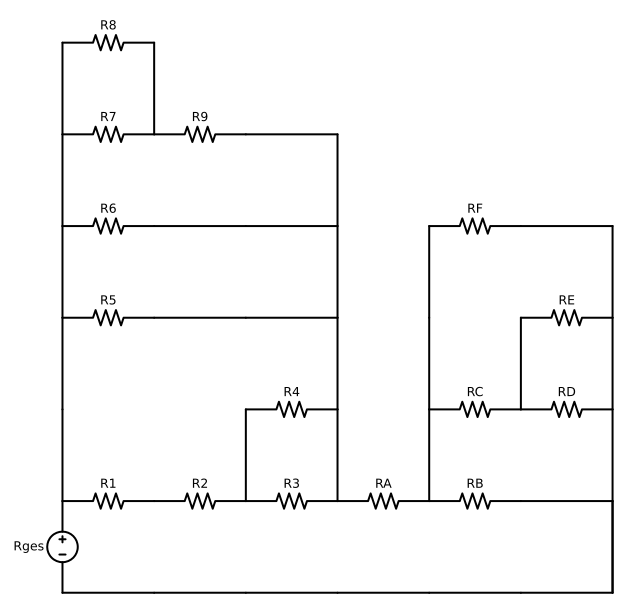
\includegraphics[width=\textwidth]{circuit2.png}

\subsection{Aufgabe 1}

\includegraphics[width=0.5\textwidth]{circuit3.png}

\begin{tabular}{p{.5\textwidth}p{.5\textwidth}}
\raggedright
\begin{verbatim}
// 1
Rges, S
    U: 24
R1
R23

R23, P
R2
R3

R2, R
    R: 40

R3, R
    R: 60
    I: 0.3
\end{verbatim}   &
\raggedleft
\begin{verbatim}
Rges, Reihenschaltung
    R: 32.0Ohm
    U: 24.0V
    I: 0.75A

R1, Widerstand
    R: 8.0Ohm
    U: 6.0V
    I: 0.75A

R23, Parallelschaltung
    R: 24.0Ohm
    U: 18.0V
    I: 0.75A

R2, Widerstand
    R: 40.0Ohm
    U: 18.0V
    I: 0.45A

R3, Widerstand
    R: 60.0Ohm
    U: 18.0V
    I: 0.3A
\end{verbatim}
\end{tabular}

\subsection{Aufgabe 2}

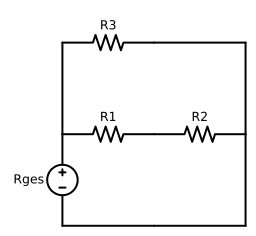
\includegraphics[width=0.5\textwidth]{circuit4.png}

\begin{tabular}{p{.5\textwidth}p{.5\textwidth}}
\raggedright
\begin{verbatim}

// 2
Rges, P
    I: 0.7
R12
R3

R12, S
R1
R2

R1, R
    R: 20

R2, R
    R: 40
    U: 8

\end{verbatim}   &
\raggedleft
\begin{verbatim}

Rges, Parallelschaltung
    R: 17.143 Ohm
    U: 12.0V
    I: 0.7A

R12, Reihenschaltung
    R: 60.0 Ohm
    U: 12.0V
    I: 0.2A

R1, Widerstand
    R: 20.0 Ohm
    U: 4.0V
    I: 0.2A

R2, Widerstand
    R: 40.0 Ohm
    U: 8.0V
    I: 0.2A

R3, Widerstand
    R: 24.0 Ohm
    U: 12.0V
    I: 0.5A

\end{verbatim}
\end{tabular}

\subsection{Aufgabe 3}

\includegraphics[width=0.5\textwidth]{circuit5.png}

\begin{tabular}{p{.5\textwidth}p{.5\textwidth}}
\raggedright
\begin{verbatim}

// 3
Rges, S
    I: 8
R12
R3

R12, P
R1
R2

R1, R
    I: 3

R2, R
    R: 2

R3, R
    R: 2

\end{verbatim}   &
\raggedleft
\begin{verbatim}

Rges, Reihenschaltung
    R: 3.25 Ohm
    U: 26.0V
    I: 8.0A

R12, Parallelschaltung
    R: 1.25 Ohm
    U: 10.0V
    I: 8.0A

R1, Widerstand
    R: 3.333 Ohm
    U: 10.0V
    I: 3.0A

R2, Widerstand
    R: 2.0 Ohm
    U: 10.0V
    I: 5.0A

R3, Widerstand
    R: 2.0 Ohm
    U: 16.0V
    I: 8.0A

\end{verbatim}
\end{tabular}

\subsection{Aufgabe 4}

\includegraphics[width=0.5\textwidth]{circuit6.png}

\begin{tabular}{p{.5\textwidth}p{.5\textwidth}}
\raggedright
\begin{verbatim}

// 4
Rges, P
    U: 42
U1
U23

U1, R
    R: 2.8

U23, S
R2
R3

R2, R
    U: 12

R3, R
    R: 1.25

\end{verbatim}   &
\raggedleft
\begin{verbatim}

Rges, Parallelschaltung
    R: 1.077 Ohm
    U: 42.0V
    I: 39.0A

U1, Widerstand
    R: 2.8 Ohm
    U: 42.0V
    I: 15.0A

U23, Reihenschaltung
    R: 1.75 Ohm
    U: 42.0V
    I: 24.0A

R2, Widerstand
    R: 0.5 Ohm
    U: 12.0V
    I: 24.0A

R3, Widerstand
    R: 1.25 Ohm
    U: 30.0V
    I: 24.0A


\end{verbatim}
\end{tabular}

\subsection{Aufgabe 16}

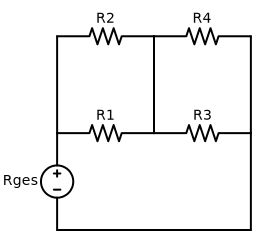
\includegraphics[width=0.5\textwidth]{circuit7.png}

\begin{tabular}{p{.5\textwidth}p{.5\textwidth}}
\raggedright
\begin{verbatim}

// 16
Rges, S
    I: 20
R12
R34

R12, P
R1
R2

R1, R
    U: 10

R2, R
    I: 5

R34, P
R3
R4

\end{verbatim}   &
\raggedleft
\begin{verbatim}

Rges, Reihenschaltung
    R: 0.9 Ohm
    U: 18.0V
    I: 20.0A

R12, Parallelschaltung
    R: 0.5 Ohm
    U: 10.0V
    I: 20.0A

R1, Widerstand
    R: 0.667 Ohm
    U: 10.0V
    I: 15.0A

R2, Widerstand
    R: 2.0 Ohm
    U: 10.0V
    I: 5.0A

R34, Parallelschaltung
    R: 0.4 Ohm
    U: 8.0V
    I: 20.0A

R3, Widerstand
    R: 0.667 Ohm
    U: 8.0V
    I: 12.0A

R4, Widerstand
    R: 1.0 Ohm
    U: 8.0V
    I: 8.0A

\end{verbatim}
\end{tabular}

\subsection{Aufgabe 7}

\includegraphics[width=0.5\textwidth]{circuit8.png}

\begin{tabular}{p{.5\textwidth}p{.5\textwidth}}
\raggedright
\begin{verbatim}

// 7
Rges, P
    U: 42
R12
R34

R12, S
R1
R2

R34, S
R3
R4

R1, R
    R: 1

R2, R
    R: 2

\end{verbatim}   &
\raggedleft
\begin{verbatim}

Rges, Parallelschaltung
    R: 2.1 Ohm
    U: 42.0V
    I: 20.0A

R12, Reihenschaltung
    R: 3.0 Ohm
    U: 42.0V
    I: 14.0A

R1, Widerstand
    R: 1.0 Ohm
    U: 14.0V
    I: 14.0A

R2, Widerstand
    R: 2.0 Ohm
    U: 28.0V
    I: 14.0A

R34, Reihenschaltung
    R: 7.0 Ohm
    U: 42.0V
    I: 6.0A

R3, Widerstand
    R: 3.0 Ohm
    U: 18.0V
    I: 6.0A

R4, Widerstand
    R: 4.0 Ohm
    U: 24.0V
    I: 6.0A

\end{verbatim}
\end{tabular}

\newpage
\section{Quellcode}

Den gesamten Quellcode, auch den der Website, finden Sie auf \href{https://github.com/HeIIow2/physik_schaltkreise}{\underline{Github}} unter Creative Commons Lizensiert.

\subsection{GUI}

\begin{lstlisting}

import read_circuit

import tkinter as tk
from tkinter import filedialog, Canvas
import os
from PIL import Image, ImageTk

class InputFrame:
    def __init__(self, root):
        self.root = root
        self.fg_color = '#fff'
        self.bg_color = '#bbb'

        self.root.config(bg=self.bg_color)

        self.string = ""
        self.file_name = os.getcwd()

        # Eingabe
        self.open_file_dialog_button = tk.Button(self.root, text=self.file_name, command=self.file_dialog, bg=self.fg_color)
        self.open_file_dialog_button.grid(row=0, column=0, sticky="NSEW", padx=5, pady=5)

        self.text = tk.Text(self.root, height=20, width=30, undo=True, relief=tk.FLAT)
        self.text.grid(row=1, column=0, sticky="NS", padx=5)
        self.root.rowconfigure(1, weight=2)

        self.calc_button = tk.Button(self.root, text="calculate and render", command=self.calculate)
        self.calc_button.grid(row=2, column=0, sticky="EWS", padx=5, pady=5)

        # Zeigt den Schaltplan am Ende
        self.schematic = tk.Label(self.root, bg=self.bg_color)
        self.schematic.grid(row=0, column=1, rowspan=3, sticky="NSEW", padx=5, pady=5)
        self.root.columnconfigure(1, weight=2)

        # Ausgabe
        self.output_label = tk.Label(self.root, text="Ausgabe", bg=self.fg_color)
        self.output_label.grid(row=0, column=2, sticky="NEW", padx=5, pady=5)

        self.output_text = tk.Text(self.root, height=20, width=30, state="disabled", relief=tk.FLAT)
        self.output_text.grid(row=1, column=2, rowspan=2, sticky="NS", padx=5, pady=(0, 5))

        self.set_text()

    def set_text(self):
        if len(self.file_name) > 45:
            display_file_name = "..." + self.file_name[-42:]
            self.open_file_dialog_button.config(text=display_file_name)

    def file_dialog(self):
        file = tk.filedialog.askopenfile(mode="r", initialdir=os.getcwd())
        if file is None:
            return
        self.file_name = file.name
        self.set_text()
        self.string = file.read()
        self.text.delete('1.0', tk.END)
        self.text.insert(tk.END, self.string)

    def calculate(self):
        print(self.root.winfo_width(), self.root.winfo_height())

        save_to_str = self.file_name.split("/")[-1].split(".")[0]

        circuit = read_circuit.Circuit(string=self.string, save_to=save_to_str)

        img = Image.open(f'graphics/png/{save_to_str}.png')

        im_width, im_height = img.size
        elm_width, elm_height = self.schematic.winfo_width(), self.schematic.winfo_height()
        if im_width/elm_width > im_height/elm_height:
            ratio = im_height/im_width
            im_height = elm_width * ratio
            im_width = elm_width
        elif im_width/elm_width < im_height/elm_height:
            ratio = im_width/im_height
            im_width = elm_height * ratio
            im_height = elm_height
        img = img.resize((int(im_width), int(im_height)))

        self.tk_img = ImageTk.PhotoImage(img)

        self.schematic.config(image=self.tk_img)
        self.output_text.configure(state='normal')
        self.output_text.delete('1.0', tk.END)
        self.output_text.insert(tk.END, circuit.output)
        self.output_text.configure(state='disabled')


root = tk.Tk()
root.title("Schaltplan CLars Noack")
# root.state("zoomed")
root.geometry("800x400")

input_frame = tk.Frame(root)
input_frame.grid(row=0, column=0)
InputFrame(root)

root.mainloop()


\end{lstlisting}

\subsection{die Adjazenzliste verarbeiten}
\label{subsec:verarbeitung}

\begin{lstlisting}

import re
import circuits


class Circuit:
    def __init__(self, path="", string="", save_to=""):
        file_str = ""

        if path != "":
            with open(path, "r") as circuit_file:
                string = circuit_file.read()

        lines = string.split("\n")
        for line in lines:
            x = re.findall("^//", line)
            if not x:
                file_str += line + "\n"

        connection_list = file_str.split("\n\n")
        for i, connection in enumerate(connection_list):
            temp_connections = connection.split("\n")
            connections = []
            for connection_ in temp_connections:
                if connection_ != "":
                    connections.append(connection_)
            connection_list[i] = connections

        elements_dict = {}

        root_name = ""

        for connection in connection_list:
            connection[0] = connection[0].replace(" ", "")
            name, type_ = connection[0].split(",")

            if root_name == "":
                root_name = name

            values_dict = {"U": -1, "R": -1, "I": -1}
            values = []
            child_names = []
            for attribute in connection[1:]:
                if re.findall("^    ", attribute) or re.findall("^\t", attribute):
                    attribute = attribute.replace(" ", "").replace("\t", "")
                    values.append(attribute)
                else:
                    child_names.append(attribute)

            for value in values:
                key = value[0].upper()
                values_dict[key] = float(value[2:])

            elements_dict[name] = [child_names,
                                   circuits.Element(name, type_, voltage=values_dict["U"], resistance=values_dict["R"],
                                                    current=values_dict["I"])]

        for elem_key in list(elements_dict):
            for child_name in elements_dict[elem_key][0]:
                if child_name in elements_dict:
                    elements_dict[elem_key][1].add_child(elements_dict[child_name][1])
                else:
                    elements_dict[elem_key][1].add_child(circuits.Element(child_name, "r"))

        elements_dict[root_name][1].draw_as_root(save_to=save_to)
        for i in range(10):
            elements_dict[root_name][1].compute()

        self.output = elements_dict[root_name][1].output_values()


if __name__ == '__main__':
    Circuit("circuits/circuit2.cd")

\end{lstlisting}

\subsection{die Logik der Knoten}
\label{subsec:berechnung}

\begin{lstlisting}

import schemdraw
import schemdraw.elements as elm
schemdraw.use('svg')


class Element:
    def __init__(self, name: str, type_str: str, resistance=-1.0, voltage=-1.0, current=-1.0):
        type_str = type_str.lower()
        types = {
            "r": 0,
            "s": 1,
            "p": 2
        }
        self.type = types[type_str]
        self.name = name

        self.resistance = float(resistance)
        self.voltage = float(voltage)
        self.current = float(current)

        self.child_Elements = []

        self.on_change()


    def ohmsches_gesetzt(self):
        if self.resistance != -1 and self.current != -1 and self.voltage == -1:
            self.voltage = self.resistance * self.current
            return

        if self.voltage != -1 and self.resistance != -1 and self.current == -1:
            if self.resistance != 0:
                self.current = self.voltage / self.resistance
            else:
                print(f"Der Widerstand bei {self.name} ist 0.")
            return

        if self.voltage != -1 and self.current != -1 and self.resistance == -1:
            if self.current != 0:
                self.resistance = self.voltage / self.current
            else:
                print(f"Die Stromspannung bei {self.name} ist 0.")
            return

        # wenn alle Werte vorhanden sind, werden diese ueberprueft
        if self.voltage != -1 and self.current != -1 and self.resistance != -1:
            if int(self.voltage) != int(self.resistance * self.current):
                print(f"Spannung[{self.resistance}] != Widerstand[{self.resistance}] * Staerke[{self.current}]")

    def maschen_knoten_children(self):
        # wenn der Richtige wert bei diesem Objekt existiert, fuege ihn bei den Kindern hinzu.

        if len(self.child_Elements) == 0:
            return

        if self.type == 1:
            # Maschenregel
            if self.current == -1:
                return

            for child in self.child_Elements:
                child.set_current(self.current)
            return

        if self.type == 2:
            # Knotenregel
            if self.voltage == -1:
                return

            for child in self.child_Elements:
                child.set_voltage(self.voltage)
            return

    def maschen_knoten_self(self):
        # wenn der Richtige wert bei den Kindern existiert, fuege ihn bei sich selbst.

        if len(self.child_Elements) == 0:
            return

        if self.type == 1:
            # Maschenregel
            for child in self.child_Elements:
                if child.current != -1:
                    self.set_current(child.current)
                    return
            return

        if self.type == 2:
            # Knotenregel
            for child in self.child_Elements:
                if child.voltage != -1:
                    self.set_voltage(child.voltage)
            return

    def set_voltage(self, voltage):
        if self.voltage != -1:
            return -1
        self.voltage = voltage
        self.on_change()

    def set_current(self, current):
        if self.current != -1:
            return
        self.current = current
        self.on_change()

    def set_resistance(self, resistance):
        if self.resistance != -1:
            return -1
        self.resistance = resistance
        self.on_change()

    def on_change(self):
        self.ohmsches_gesetzt()
        self.maschen_knoten_children()

    def compute(self):
        if len(self.child_Elements) == 0:
            return
        if self.type == 0:
            return

        # get the amount of unknown values
        unknown_voltage = 0
        unknown_current = 0
        unknown_resistance = 0
        for child in self.child_Elements:
            if child.voltage == -1:
                unknown_voltage += 1
                missing_voltage_elem = child
            if child.current == -1:
                unknown_current += 1
                missing_current_elem = child
            if child.resistance == -1:
                unknown_resistance += 1
                missing_resistance_elem = child

        if self.type == 1:
            # Reihenschaltung
            if unknown_resistance == 0:
                total_resistance = 0
                for child in self.child_Elements:
                    total_resistance += child.resistance
                self.set_resistance(total_resistance)

            elif unknown_resistance == 1 and self.resistance != -1:
                total_resistance = 0
                for child in self.child_Elements:
                    if child.resistance != -1:
                        total_resistance += child.resistance
                missing_resistance_elem.set_resistance(self.resistance - total_resistance)

            if unknown_voltage == 0:
                total_voltage = 0
                for child in self.child_Elements:
                    total_voltage += child.voltage
                self.set_voltage(total_voltage)

            elif unknown_voltage == 1 and self.voltage != -1:
                total_voltage = 0
                for child in self.child_Elements:
                    if child.voltage != -1:
                        total_voltage += child.voltage
                missing_voltage_elem.set_voltage(self.voltage - total_voltage)


        elif self.type == 2:
            # Parallelschaltung
            if unknown_current == 0:
                total_current = 0
                for child in self.child_Elements:
                    total_current += child.current
                self.set_current(total_current)

            elif unknown_current == 1 and self.current != -1:
                total_current = 0
                for child in self.child_Elements:
                    if child.current != -1:
                        total_current += child.current

                missing_current_elem.set_current(self.current - total_current)

        self.maschen_knoten_self()
        self.maschen_knoten_children()

        for child in self.child_Elements:
            child.compute()

    def output_values(self, return_str=""):
        type_descriptions = ["Widerstand", "Reihenschaltung", "Parallelschaltung"]
        return_str += f"{self.name}, {type_descriptions[self.type]}\n"
        print(f"{self.name}, {type_descriptions[self.type]}")
        if self.resistance != -1:
            print(f"    R: {round(self.resistance, 3)}Ohm")
            return_str += f"    R: {round(self.resistance, 3)}Ohm\n"
        if self.voltage != -1:
            print(f"    U: {round(self.voltage, 3)}V")
            return_str += f"    U: {round(self.voltage, 3)}V\n"
        if self.current != -1:
            print(f"    I: {round(self.current, 3)}A")
            return_str += f"    I: {round(self.current, 3)}A\n"
        return_str += "\n"
        print("")

        if self.type == 1 or self.type == 2:
            for child in self.child_Elements:
                return_str = child.output_values(return_str=return_str)

        return return_str

    def add_child(self, child):
        self.child_Elements.append(child)
        self.maschen_knoten_self()

    def draw(self, d: schemdraw.Drawing, latest_elem):
        if self.type == 0:
            d += (latest_elem := elm.Resistor().right().label(self.name).at(latest_elem.end))

            return 1, latest_elem, 1

        if self.type == 1:
            steps = 0
            height = 1

            for child in self.child_Elements:
                r_steps, latest_elem, height = child.draw(d, latest_elem)
                steps += r_steps

            return steps, latest_elem, height

        if self.type == 2:
            steps, last, heights = self.child_Elements[0].draw(d, latest_elem)
            parallel_steps = [steps]
            parallel_heights = [heights]
            parallel_last = [last]

            for child in self.child_Elements[1:]:
                for n in range(parallel_heights[-1]):
                    d += (latest_elem := elm.Line().up().at(latest_elem.end))
                steps, last, height = child.draw(d, latest_elem)
                parallel_steps.append(steps)
                parallel_last.append(last)
                parallel_heights.append(height)

            # get max steps
            max_steps = 0
            for step in parallel_steps:
                if step > max_steps:
                    max_steps = step

            # draw rest of the circuit
            for i, latest_elem in enumerate(parallel_last):
                for n in range(max_steps - parallel_steps[i]):
                    d += (latest_elem := elm.Line().right().at(latest_elem.end))
                if i > 0:
                    for n in range(parallel_heights[i]):
                        d += (latest_elem := elm.Line().down().at(latest_elem.end))
                else:
                    latest_elem_r = latest_elem

            current_height = 0
            for heights in parallel_heights:
                current_height += heights

            return max_steps, latest_elem_r, current_height

    def draw_as_root(self, save_to=""):
        d = schemdraw.Drawing()

        d += (latest_elem := elm.SourceV().up().label(self.name))

        steps, latest_elem, height = self.draw(d, latest_elem)

        d += (latest_elem := elm.Line().down().at(latest_elem.end))
        for i in range(steps):
            d += (latest_elem := elm.Line().left().at(latest_elem.end))

        d.draw()
        if save_to == "":
            d.save('schematic.svg')
        else:
            d.save(f"graphics/png/{save_to}.png", dpi=300)
            d.save(f"graphics/{save_to}.svg")

\end{lstlisting}

\end{document}
